\documentclass{article}
\usepackage[utf8]{inputenc}

\title{Comp280 Worksheet 3}
\author{Matt Shaw - ms228668}

\usepackage{natbib}
\usepackage{graphicx}
\usepackage{hyperref}
\usepackage[none]{hyphenat}
\usepackage{color}
\definecolor{cloudwhite}{rgb}{0.9412, 0.9608, 0.8471}
\definecolor{red}{rgb}{0.6,0,0} 
\definecolor{blue}{rgb}{0,0,0.6}
\definecolor{green}{rgb}{0,0.8,0}
\definecolor{cyan}{rgb}{0.0,0.6,0.6}
\usepackage{listings}
\lstset{
language=csh,
basicstyle=\tiny\ttfamily,
numbers=left,
numberstyle=\tiny,
numbersep=5pt,
tabsize=2,
extendedchars=true,
breaklines=true,
frame=b,
stringstyle=\color{blue}\ttfamily,
showspaces=false,
showtabs=false,
xleftmargin=17pt,
framexleftmargin=17pt,
framexrightmargin=5pt,
framexbottommargin=4pt,
morecomment=[l]{//}, %use comment-line-style!
morecomment=[s]{/*}{*/}, %for multiline comments
showstringspaces=false,
morekeywords={ abstract, event, new, struct, as, explicit, null, switch, base, extern, object, this, bool, false, operator, throw,
break, finally, out, true, byte, fixed, override, try, case, float, params, typeof, catch, for, private, uint, char, foreach, protected, ulong,
checked, goto, public, unchecked, class, if, readonly, unsafe, const, implicit, ref, ushort, continue, in, return, using, decimal, int, sbyte, virtual,
default, interface, sealed, volatile, delegate, internal, short, void, do, is, sizeof, while, double, lock, stackalloc, else, long, static,
enum, namespace, string},
keywordstyle=\color{cyan},
identifierstyle=\color{red},
}
\usepackage{tikz}
\def\Csharp{C\tikz[x=1em,y=\baselineskip]%
  \draw (0.125,0.15) -- ++(0.15,0.5)%
        (0.325,0.15) -- ++(0.15,0.5)%
        (0.05,0.3) -- ++(0.45,0.0)%
        (0.1,0.5) -- ++(0.45,0.0);}

\begin{document}

\maketitle

\section{Introduction}
For this assignment, I'm going to be using a project I worked on, which can be found here: \url{https://github.com/ThatVoidUpdate/TestProject}. \\
It is a simple effect, where you can fire out a load of bullets, then right click on an object to summon all the bullets to that object. I believe that it is pretty unoptimised, and while the frames per second is still above 60, it was written in a relatively unoptimised way, and as such is a good candidate for this task.
\begin{center}
    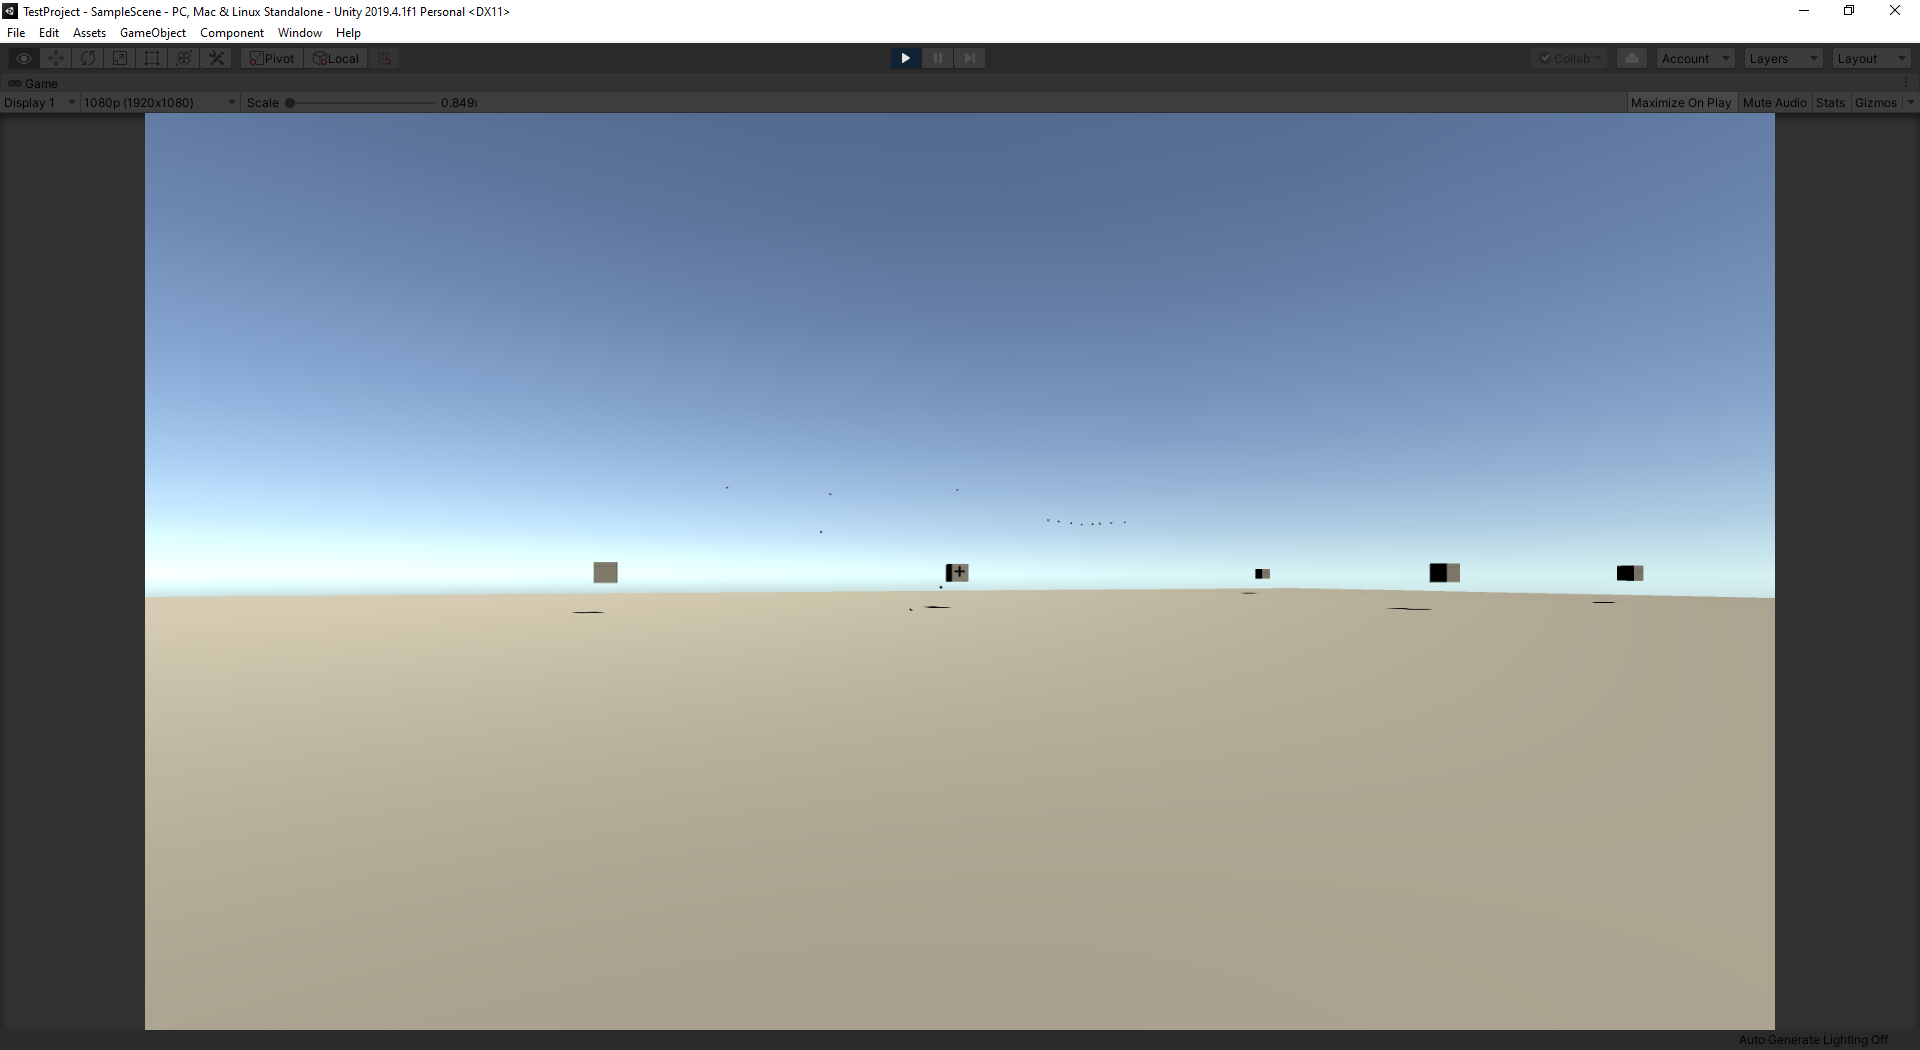
\includegraphics[width=\textwidth]{Images/Example.png}\\
    An example of the effect in action, though it may be hard to see\\
\end{center}
The first thing to do is to get a first look at the performance of the project using the profiler.
\begin{center}
    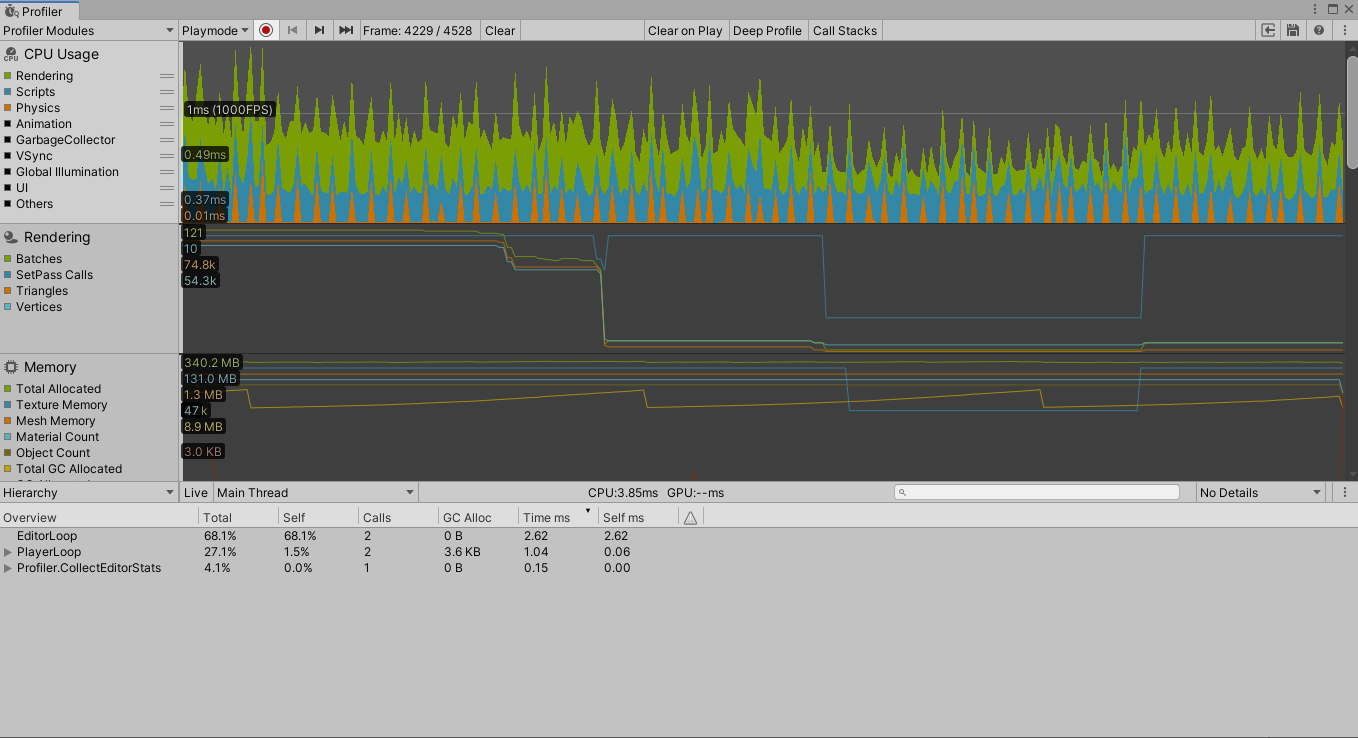
\includegraphics[width=\textwidth]{Images/FirstProfile.png}
    The first profiler view
\end{center}
In this view, I have turned off a load of the cpu views, leaving just the main 3 contributors, those being rendering, scripts and physics.
The rendering stage deals with displaying the game on screen. Slow performance there could be caused by badly optimised culling, drawing objects when they dont need to be drawn, and potentially repeated changes in materials.
Scripts is all of the scripts ive added to objects. Reduced performance there is usually down to poor programming descisions, like calling expensive functions every frame.
Finally, physics is all of the rigidbody and collider interactions. If there are many physics objects in the scene, this would contribute to decreased speed.\\
The first thing to focus on, as it is usually a large contributor to slow performance, is scripts. 
\begin{center}
    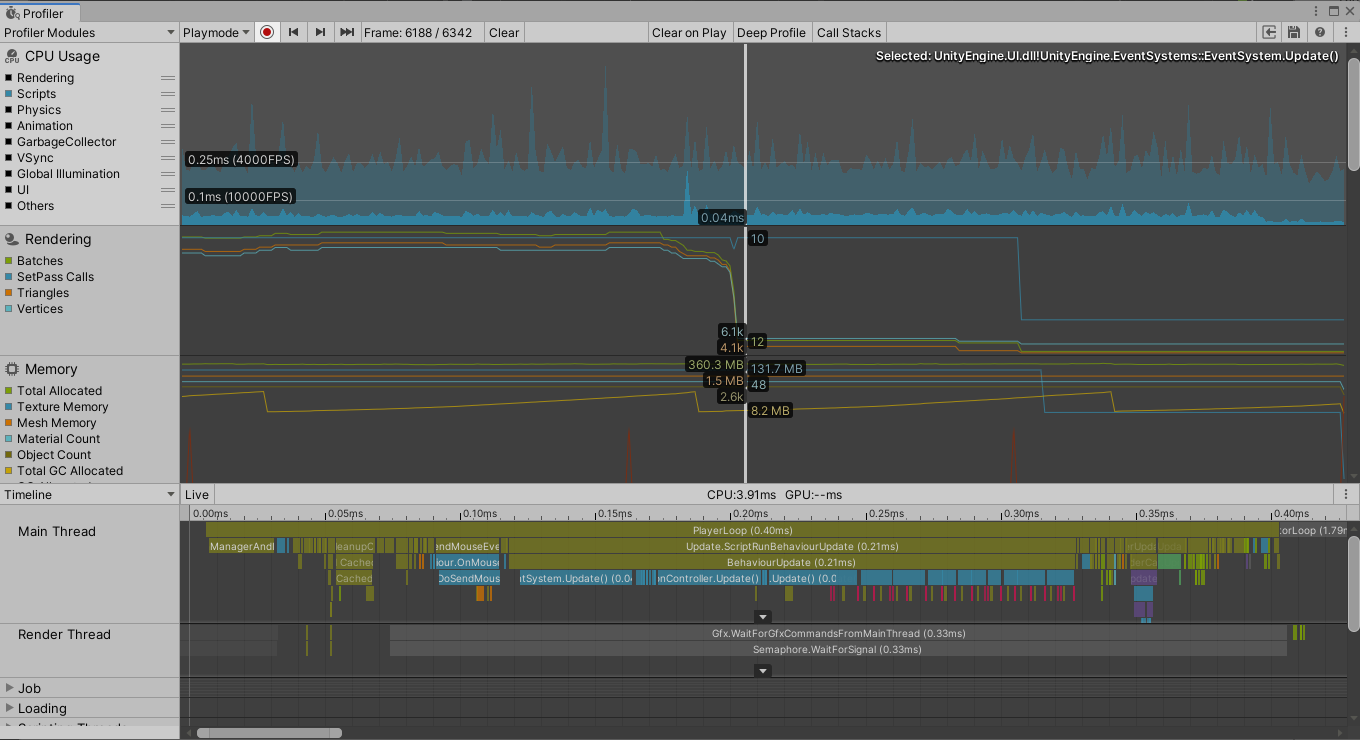
\includegraphics[width=\textwidth]{Images/FirstScripts.png}
    A view of an average frame
\end{center}
Looking at the Timeline view at the bottom, we can see that the main thing happening each frame is the Update method calls. If we look first at my code specifically, the first method is called on the PlayerController, and it is taking a comparatively long time (0.04ms). This seems like a good candidate to look at first.

Here is a listing of the FirstPersonController script
\begin{lstlisting}[language={[Sharp]C}, label={Script}]
    public class FirstPersonController : MonoBehaviour
    {
        [Header("Speeds")]
        public float ForwardSpeed;
        public float SidewaysSpeed;
    
        [Header("Mouse Sensitivity")]
        public float MouseSensitivityX;
        public float MouseSensitivityY;
    
        [Space]
        public bool AirControl = true;
        public float JumpForce;
    
        private Vector3 MovementVector;
        private float HeadAngle = 0;
        // Start is called before the first frame update
        void Start()
        {        
            Cursor.lockState = CursorLockMode.Locked;
            Cursor.visible = false;
        }
    
        // Update is called once per frame
        void Update()
        {
            CharacterController controller = GetComponent<CharacterController>();
            MovementVector.x = Input.GetAxis("Horizontal") * SidewaysSpeed;
            MovementVector.z = Input.GetAxis("Vertical") * ForwardSpeed;
            if (Input.GetButtonDown("Jump"))
            {
                MovementVector.y = JumpForce;
            }
    
            MovementVector.y -= -Physics.gravity.y * Time.deltaTime;
    
            if (controller.isGrounded || (!controller.isGrounded && AirControl))
            {
                controller.Move(transform.TransformDirection(MovementVector * Time.deltaTime));
            }
    
    
    
            transform.Rotate(new Vector3(0, Input.GetAxis("Mouse X") * MouseSensitivityX, 0));
            HeadAngle = Mathf.Clamp(HeadAngle + (Input.GetAxis("Mouse Y") * MouseSensitivityY), -90, 90);
    
            Camera.main.transform.localEulerAngles = new Vector3(HeadAngle, 0, 0);
    
            if (Input.GetAxis("Cancel") == 1)
            {
                Cursor.lockState = CursorLockMode.None;
                Cursor.visible = true;
            }
    
        }
    }
\end{lstlisting}
The main things that are important are lines 27 and 47. Line 27 runs an expensive \lstinline[basicstyle=\footnotesize]{GetComponent<>()} method. These should ideally only be run in the Start or Awake methods, as they can take a very logn time to run.
The other problem is in line 47, with a call to \lstinline[basicstyle=\footnotesize]{Camera.main}. This checks every GameObject in the scene to try and find the camera tagged with MainCamera. This should also be moved to the start method if possible.\\
Making these changes results in this code:
\begin{lstlisting}[language={[Sharp]C}, label={Script}]
public class FirstPersonController : MonoBehaviour
{
    [Header("Speeds")]
    public float ForwardSpeed;
    public float SidewaysSpeed;

    [Header("Mouse Sensitivity")]
    public float MouseSensitivityX;
    public float MouseSensitivityY;

    [Space]
    public bool AirControl = true;
    public float JumpForce;

    private Vector3 MovementVector;
    private float HeadAngle = 0;

    private Camera camera;
    private CharacterController controller;
    // Start is called before the first frame update
    void Start()
    {        
        Cursor.lockState = CursorLockMode.Locked;
        Cursor.visible = false;

        camera = Camera.main;
        controller = GetComponent<CharacterController>();
    }

    // Update is called once per frame
    void Update()
    {
        
        MovementVector.x = Input.GetAxis("Horizontal") * SidewaysSpeed;
        MovementVector.z = Input.GetAxis("Vertical") * ForwardSpeed;
        if (Input.GetButtonDown("Jump"))
        {
            MovementVector.y = JumpForce;
        }

        MovementVector.y -= -Physics.gravity.y * Time.deltaTime;

        if (controller.isGrounded || (!controller.isGrounded && AirControl))
        {
            controller.Move(transform.TransformDirection(MovementVector * Time.deltaTime));
        }

        transform.Rotate(new Vector3(0, Input.GetAxis("Mouse X") * MouseSensitivityX, 0));
        HeadAngle = Mathf.Clamp(HeadAngle + (Input.GetAxis("Mouse Y") * MouseSensitivityY), -90, 90);

        camera.transform.localEulerAngles = new Vector3(HeadAngle, 0, 0);

        if (Input.GetAxis("Cancel") == 1)
        {
            Cursor.lockState = CursorLockMode.None;
            Cursor.visible = true;
        }

    }
}
\end{lstlisting}
Making these changes reduces the time takes to 0.034ms, 85\% of the original speed. While this is not a huge saving, if there were more components on the character, the \lstinline[basicstyle=\footnotesize]{GetComponent<>()} call would take much longer, and if there are more objects in the scene, the \lstinline[basicstyle=\footnotesize]{Camera.main} call would take longer. It is always best to move these expensive calls to the Start method where possible.
\begin{center}
    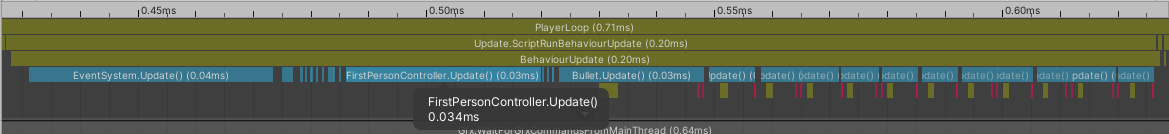
\includegraphics[width=\textwidth]{Images/ControllerFixed.png}
\end{center}

The next thing to look at is the bullet script. 
\begin{center}
    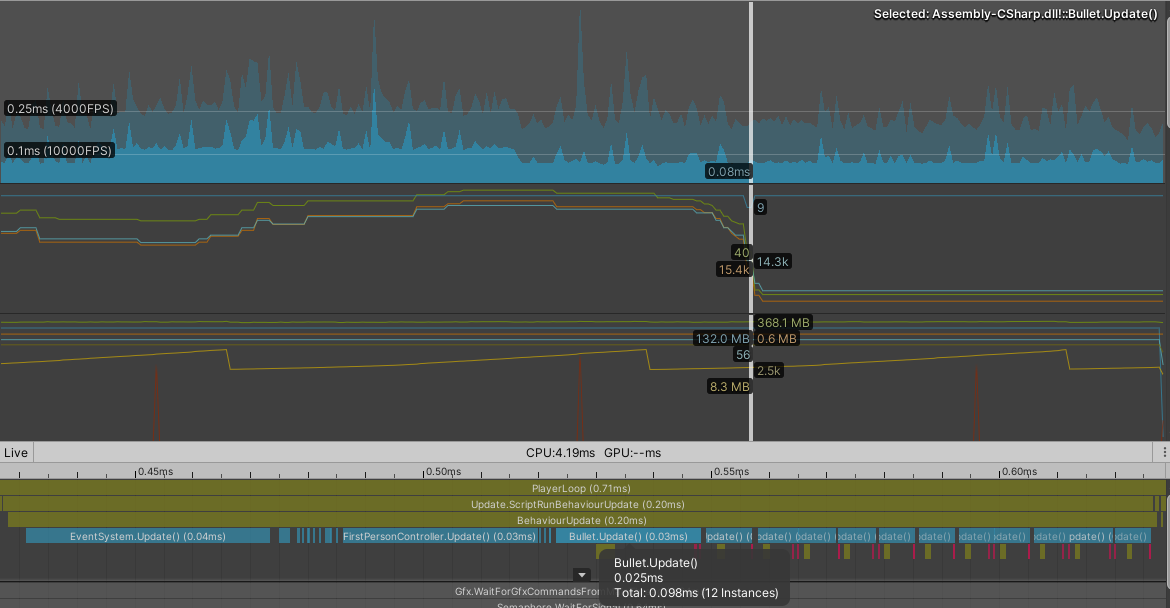
\includegraphics[width=\textwidth]{Images/BulletStart.png}
\end{center}
Looking at the histogram at the top with the bullet update method selected, we can see that it makes up a large proportion of the frame budget.
We can also see that it makes a call to a lower function, and provokes a memory allocation. 
This is the code for the bullets:
\begin{lstlisting}[language={[Sharp]C}, label={Script}]
public class Bullet : MonoBehaviour
{
    public float speed;

    Vector3 Direction;

    // Start is called before the first frame update
    void Start()
    {
        Direction = transform.forward;
    }

    // Update is called once per frame
    void Update()
    {
        GetComponent<Rigidbody>().velocity = Direction * speed;

        if (FindObjectsOfType<Gun>()[0].IsAttracting)
        {
            Direction = (FindObjectsOfType<Gun>()[0].AttractingObject.transform.position - transform.position).normalized;
        }
    }
}
\end{lstlisting}
Here the main culprits are lines 16, 18 and 20. These are all calls to expensive methods, and 18 and 20 especially since \lstinline[basicstyle=\footnotesize]{FindObjectsOfType<>()} will iterate over every component of every gameobject, which is extremely inefficient in larger projects.
Making changes to the code to move those expensive calls to the Start method gives this improved code.
\begin{lstlisting}[language={[Sharp]C}, label={Script}]
    public class Bullet : MonoBehaviour
{
    public float speed;

    Vector3 Direction;

    private Rigidbody rb;
    private Gun gun;

    // Start is called before the first frame update
    void Start()
    {
        Direction = transform.forward;
        rb = GetComponent<Rigidbody>();
        gun = FindObjectOfType<Gun>();
    }

    // Update is called once per frame
    void Update()
    {
        rb.velocity = Direction * speed;

        if (gun.IsAttracting)
        {
            Direction = (gun.AttractingObject.transform.position - transform.position).normalized;
        }
    }
}
\end{lstlisting}
Running the profiler again shows a roughly 25x increase in speed. This shows just how intensive the \lstinline[basicstyle=\footnotesize]{FindObjectsOfType<>()} method can be.

\begin{center}
    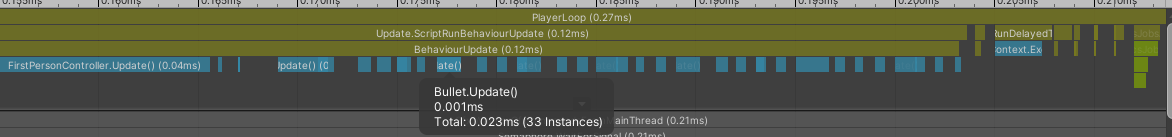
\includegraphics[width=\textwidth]{Images/BulletFixed.png}
\end{center}

Continuing to look at the profiler again, we can see many small slices in the update section.

\begin{center}
    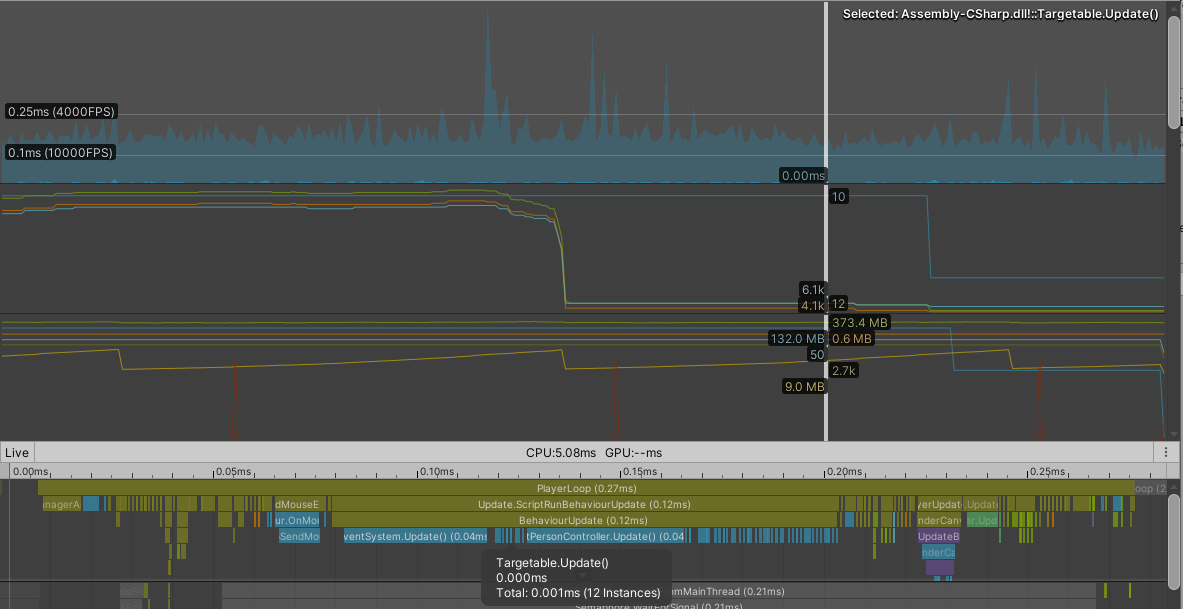
\includegraphics[width=\textwidth]{Images/TargetableStart.png}
\end{center}

Clicking on them shows that they are from the Targetable script, which is odd since they dont do anything each frame. Looking at their code quickly reveals the problem.

\begin{lstlisting}[language={[Sharp]C}, label={Script}]
public class Targetable : MonoBehaviour
{
    // Start is called before the first frame update
    void Start()
    {
        
    }

    // Update is called once per frame
    void Update()
    {
        
    }

    private void OnMouseEnter()
    {
        FindObjectsOfType<Gun>()[0].AttractingObject = this.gameObject;
    }

    private void OnMouseExit()
    {
        FindObjectsOfType<Gun>()[0].AttractingObject = null;
    }
}
\end{lstlisting}
The problem here is not obvious at first glace, as usually the \Csharp {} compiler would optimise away empty functions. However, Unity will keep them around during compilation, and they are still called, due to how the engine works internally. Empty Unity functions are still called whenever they would usually be called, which can cause a performance hit if it is done a lot.
These functions can be removed for a boost, like this:

\begin{lstlisting}[language={[Sharp]C}, label={Script}]
public class Targetable : MonoBehaviour
{
    private void OnMouseEnter()
    {
        FindObjectsOfType<Gun>()[0].AttractingObject = this.gameObject;
    }

    private void OnMouseExit()
    {
        FindObjectsOfType<Gun>()[0].AttractingObject = null;
    }
}
\end{lstlisting}

After running the profiler yet again, we can see that Targetable is no longer involved in the Update method. Again, this did not cause a particularly large improvement in this project, but it could become a problem in larger projects.

\begin{center}
    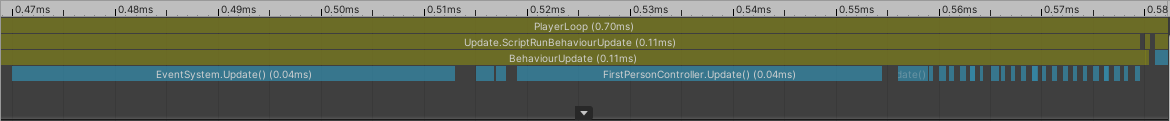
\includegraphics[width=\textwidth]{Images/TargetableFixed.png}
\end{center}


\end{document}